% This Source Code Form is subject to the terms of the Mozilla Public
% License, v. 2.0. If a copy of the MPL was not distributed with this
% file, You can obtain one at http://mozilla.org/MPL/2.0/.
%
% Copyright (c) 2011-2019 ETH Zurich.

\begin{chapter}{Trace Partitioning}
	\label{chapter:TracePartitioning}
	This chapter describes the trace partitioning abstract domain as it is presented in \cite{mauborgne:rival07, mauborgne:rival05} in detail. The theory is necessary in order to understand the implementation described in Chapter \ref{chapter:Extension}. Once more, the focus of the discussion lies on intuition rather than on rigorous formal definitions. All relevant proofs and further examples can be found in the referenced paper.\\

	Static analysis with abstract interpretation as presented in Section \ref{section:StaticAnalysis} has proven to be both flexible and efficient. There are, however, cases where the approximation of reachable states provided by the fixed point computation is too coarse to produce meaningful results. This is the case when the proof of a property relies, for example, on the way a state is reached, a piece of information that is completely discarded during the standard analysis.

	A possible remedy would be to analyze a more precise approximation of the concrete semantics. Unfortunately, simply abandoning the reachable state semantics in favor of a more precise abstraction (e.g. the trace semantics) has so far turned out to come at too high a price in terms of complexity.

	Trace partitioning is an attempt at finding the middle ground between the prohibitive complexity of discerning traces and the overly simplistic view of the reachable state semantics. It does so by effectively partitioning reachable states based on \emph{some} decisions made along the control flow. The theory is very general and fits well within the abstract interpretation framework and can be formalized as an abstract domain.

	% REFINED SEMANTICS

	\begin{section}{Refined Semantics}
		Before talking about how the partitioning works, it is important to know what exactly a partitioning is and how it can be used to refine the collecting semantics.

		\begin{definition}[Covering and Partition]
			\label{definition:coveringpartition}
			A mapping $\delta: E \to \wp(S)$ is said to be a covering of $S$ if
			\begin{equation}
				S = \bigcup_{e \in E} \delta(e).
			\end{equation}
			If additionally all elements of $E$ produce disjunct images in $S$, i.e.
			\begin{equation}
				\forall e, e' \in E, \ e \neq e' \land \delta(e) \cap \delta(e') = \varnothing,
			\end{equation}
			$\delta$ is called a partitioning of $S$.
		\end{definition}

		The name trace partitioning is misleading since the theory does not depend on partitions but is sound with coverings as well. Nonetheless, for the sake of simplicity, the further discussion will distinguish between the two only when necessary.

		The underlying idea of trace partitioning is to refine the collecting semantics using partitions. To illustrate how, it helps to take another look at the whole abstraction process from the concrete semantics of a program to the abstract state. Since Galois connections, as defined by Cousot \& Cousot, are composable, the abstraction can be split into two parts

		\begin{align}
			\label{equation:ReachabilityAbstraction1}
			\concrete{P} \galois{\alpha_C}{\gamma_C} &\collecting{P} \galois{\alpha_D}{\gamma_D} D.
		\end{align}

		The two steps are

		\begin{itemize}
			\item the abstraction of the concrete semantics \concrete{P} to the collecting semantics \collecting{P} followed by
			\item the abstraction of the reachable states of the collecting semantics to some other abstract domain $D$.
		\end{itemize}

		The first abstraction can be extended to include a partitioning $\delta: E \to \concrete{P}$. The two steps can then be rewritten as

		\begin{align}
			\label{equation:partitionedreachabilityabstraction1}
			\concrete{P} \galois{\alpha_\delta}{\gamma_\delta} &(E \to \concrete{P}) \galois{\alpha_D}{\gamma_D} D.
		\end{align}

		Here, $\alpha_\delta$ describes the abstraction that transforms the concrete semantics into a function that maps elements of some label set $E$ to traces of \concrete{P}. The abstraction is called partitioning abstraction and can be shown to form a Galois connection, provided that $\delta$ is in fact a covering or a partitioning. A more formal definition of the abstraction and concretization functions follows.

		\begin{definition}[Partitioning Abstraction]
			\label{definition:partitioningabstraction}
			The partitioning abstraction is defined as
			\begin{align}
				\alpha_\delta: \concrete{P} &\to (E \to \concrete{P})\\
				\sigma &\mapsto \lambda(e) \cdot \sigma \cap \delta(e) \notag
			\end{align}
			and its corresponding concretization as
			\begin{align}
				\gamma_\delta: (E \to \concrete{P}) &\to \concrete{P}\\
				\phi &\mapsto \bigcup_{e \in E} \phi(e). \notag
			\end{align}
		\end{definition}
		
		Note that so far no decision about the form of $\delta$ has been made. This leaves a large degree of freedom in designing the abstract domain. Consider, on the one hand, the partitioning that maps a unique label to each trace of \concrete{P}. This amounts to having access to the full trace semantics during the further analysis at the expense of having to deal with the accompanying complexity. On the other hand, a partitioning that collects traces ending in the same state results in the classical situation of dealing with the collecting semantics during the analysis. These are the two extremes, anywhere in between is possible. As always there is a trade-off between complexity and precision of the analysis. The fundamental difference to other approaches to this problem is that this trade-off can be managed with great flexibility using the mechanism introduced by a custom partitioning function.
		
		This extension is the foundation of trace partitioning. The rest of this chapter will be concerned with defining an appropriate partition function as well as constructing the lattice structure required for a sound abstract domain.
	\end{section}

	% PARTITIONING TRANSITION SYSTEMS

	\begin{section}{Partitioning Transition Systems}
		The extension of the traditional abstraction and the choice of the partitioning in particular leave many questions to be answered. The goal of this section is to define a useful partitioning as well as an ordering on partitions that can be used to define an abstract domain. Furthermore, it is important to introduce the notion of semantic adequacy, showing that this extension describes the same program as the original semantics.

		The underlying structure to partition is the program whose semantics is represented by the transition system. But what does it mean to partition such a system? This is probably the most complex aspect of trace partitioning. It requires an extension of the notion of transition systems presented in Definition \ref{definition:transitionsystem}.

		\begin{definition}[Partitioned System, Trivial Extension]
			\label{definition:partitionedsystem}
			A partitioned transition system $P^T$ is an extension of a transition system $P = (\Sigma, \Sigma_0, \to)$ represented as a tuple $(T, \Sigma^T, \Sigma_0^T, \to^T)$ where 
			\begin{itemize}
				\item $T$ denotes a set of tokens (or labels),
				\item $\Sigma^T = T \times \Sigma$ denotes the set of states,
				\item $\Sigma_0^T \subseteq T \times \Sigma_0$ the set of initial states and
				\item $\to^T \ \subseteq \Sigma^T \times \Sigma^T$ is the transition relation.
			\end{itemize}

			Furthermore, the trivial extension of $P$ is defined as the partitioned system with a single token $t$ (i.e. $T = \{t\}$) where all states are extended with $t$ and the extended transition relation completely ignores the newly introduced token.
		\end{definition}

		The only difference to the original transition system is that every state now comes with an additional token of some token set $T$. The token set $T$ can be thought of as a set of available labels that can be associated with states. This makes it possible to assign tokens to whole traces of $P$, effectively providing a way to define the partitioning $\delta$.

		Another way of looking at the tokens is interpreting them as an extension of the control state as it is done in the presentation of Mauborgne and Rival. The extended control state is then defined as $L^T = T \times L$, a notion which I too will use in the further presentation.

		\begin{definition}[Partitioned Semantics]
			The partitioned semantics \partitioned{P^T} of $P^T$ is described by applying the partitioning abstraction (Definition \ref{definition:partitioningabstraction}) to the concrete semantics using the partitioning
			\begin{align}
				\delta: \concrete{P} &\to (L \to \concrete{P})\\
				S &\mapsto \lambda(l) \cdot \{s \in S | \exists \sigma \in \Sigma^T, s = \langle ..., (l, \sigma) \rangle \}. \notag
			\end{align}
		\end{definition}

		In order to relate two partitioned systems $P^T$ and $P^{T'}$ that are based on the same original transition system $P$, a function $\tau: T \to T'$ relating the labels is required. This function is called forget function since it is mainly used to relate a more complicated set of labels to a simpler one by systematically ``forgetting'' information. The function is trivially extended to states, traces, and sets of traces by applying $\tau$ to the associated token, all occurring states, and all occurring traces of the set respectively.

		\begin{definition}[Coverings, Partitions, Completeness]
			For a transition system $P$ and its two extensions $P^T$ and $P^{T'}$:
			\begin{enumerate}
				\item $P^T$ is a $\tau$-covering of $P^{T'}$ if for every transition in $P^{T}$ there exists a corresponding transition in $P^{T'}$, that is
					\begin{itemize}
						\item $\Sigma_0^{T'} \subseteq \Sigma_0^T$
						\item $\forall \sigma_0 \in \Sigma^T, \ \sigma_1' \in \Sigma^{T'}, \ \tau(\sigma_0) \to^{T'} \sigma_1' \implies \exists \sigma_1 \in \Sigma^T, \ \tau(\sigma_1) = \sigma_1' \land \sigma_0 \to^T \sigma_1$.
					\end{itemize}
				\item $P^T$ is a $\tau$-partition of $P^{T'}$ if additionally the corresponding transition is unique
					\begin{itemize}
						\item $\forall \sigma' \in \Sigma_0^{T'}, \ \exists! \sigma \in \Sigma_0^T, \ \sigma' = \tau(\sigma)$
						\item $\forall \sigma_0 \in \Sigma^T, \ \sigma_1' \in \Sigma^{T'}, \ \tau(\sigma_0) \to^{T'} \sigma_1' \implies \exists! \sigma_1 \in \Sigma^T, \ \tau(\sigma_1) = \sigma_1' \land \sigma_0 \to^T \sigma_1$.
					\end{itemize}
				\item Furthermore, $P^T$ is called $\tau$-complete with respect to $P^{T'}$ if it does not contain any superfluous transitions
					\begin{itemize}
						\item $\forall \sigma \in \Sigma_0^T, \ \tau(\sigma) \in \Sigma_0^{T'}$
						\item $\forall \sigma_0, \ \sigma_1 \in \Sigma^{T}, \ \sigma_0 \to^T \sigma_1 \implies \tau(\sigma_0) \to^{T'} \tau(\sigma_1)$.
					\end{itemize}
			\end{enumerate}
		\end{definition}

			The relations ``$\tau$-complete covering'' and ``$\tau$-complete partition'' can be shown to be transitive, antisymmetric and reflexive and hence describe a partial ordering on the set of possible partitioned systems of $P$. The ordering is denoted with the $\curlyeqprec_\tau$ operator.

		\begin{definition}[Partial Ordering]
			The partial ordering $\curlyeqprec$ amongst partitioned systems $P^T$ and $P^{T'}$ based is defined as
			\begin{equation}
				P^T \curlyeqprec P^{T'} \Longleftrightarrow \exists \tau, \ P^T \curlyeqprec_\tau P^{T'}.
			\end{equation}
		\end{definition}

		Each transition system describes many partitioned transition systems that are complete coverings of itself. The most basic one is the trivial extension which therefore corresponds to the $\bot$ element of the ordering. The $\top$ element is not tractable and more of a theoretical interest. It must cover all possible complete coverings of the trivial extensions for all possible forget functions $\tau$ for all possible token sets.

		\begin{example}[Extended System]
			\label{example:extendedsystem}
			For this example, consider once more the example program from Listing \ref{listing:positivesource}. This time, only the control but not the memory state changes, the memory abstraction consists of one single element. Figure \ref{figure:positiveextendedtransitionsystem} depicts the basic transition system in \one. The labels of the nodes correspond to the control states and indicate the line number of the program. The graph \two shows the trivial extension $P^T$ with $T = \{t\}$ and the graph on the right represents a partitioning of the trivial extension with $T' = \{t_0, t_1, t_2\}$. The additional two tokens $t_1$ and $t_2$ can be thought of as a partitioning of traces depending on which conditional branch has been taken. The forget function $\tau: T' \to T$ maps all $t_i \in T'$ to $t \in T$ (i.e. it \emph{forgets} the index) and therefore the statements $P^T \curlyeqprec_\tau P^{T'}$ and $P^T \curlyeqprec P^{T'}$ hold.
			\exampleend

			\begin{figure}[t]
				\centering
				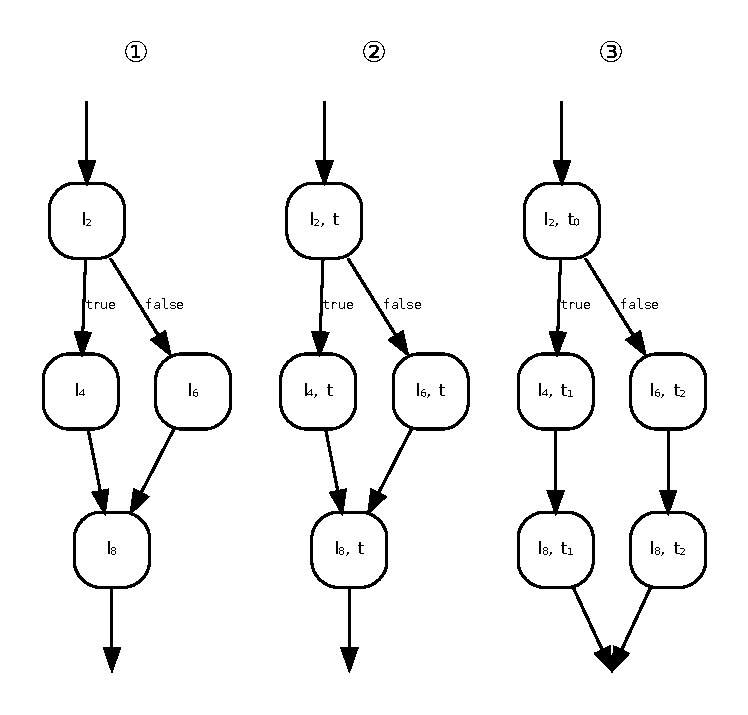
\includegraphics{Graphs/Examples_ifExampleExtendedTransitionSystem.pdf}
				\caption{Trivial Extension and Complete Partition}
				\label{figure:positiveextendedtransitionsystem}
			\end{figure}
		\end{example}

		For qualitative statements about coverings and reductions one further helper function is necessary.

		\begin{definition}[Semantic Transfer]
			\label{definition:SemanticTransfer}
			The semantic function $\Gamma_\tau$ for two extended transition systems $P^T$ and $P^{T'}$, where $P^T$ is a $\tau$-covering of $P^{T'}$, transfers a function from one system to another by associating the ``forgotten'' tokens in the covered system with the corresponding ``forgotten'' traces of the original mapping
			\begin{align}
				\Gamma_\tau: (T \to \concrete{P^T}) &\to (T' \to \concrete{P^{T'}})\\
				\phi &\mapsto \lambda(t') \cdot \bigcup\{ \tau(\phi(l)) | t \in T, \tau(t) = t' \}. \notag
			\end{align}
		\end{definition}

		Finally, this makes it possible to state the single most important theorem about partitioned transition systems.
		
		\begin{theorem}[Semantic Adequacy]
			If $P^T$ is a $\tau$-complete partitioning or $\tau$-complete covering of $P^{T'}$ the partitioned semantics is adequate (sound and complete), that is
			\begin{equation}
				\partitioned{P^{T'}} = \Gamma_\tau(\partitioned{P^T}).
			\end{equation}
		\end{theorem}

		Simply put, by partitioning a system information may be gained, but it is not possible to construct a less precise set of traces.

	\end{section}

	% TRACE PARTITIONING ABSTRACT DOMAIN

	\begin{section}{Trace Partitioning Abstract Domain}
		Now that the groundwork has been laid, it is time to put the pieces together and finally build the trace partitioning abstract domain.

		\begin{definition}[Trace Partitioning Domain]
			The trace partitioning abstract domain for a given transition system $P$ contains tuples of the form $(T, P^T, \Phi)$ where
			\begin{itemize}
				\item $T$ is a set of tokens,
				\item $P^T$ is a complete covering of $P$ and
				\item $\Phi$ is a function $\Phi: L^T \to \partitioned{P^T}$ relating partitioned control states with the partitioned traces reaching the control state.
			\end{itemize}
			The ordering can be defined as follows. For two elements $(T, P^T, \Phi) \leq (T', P^{T'}, \Phi')$ if
			\begin{itemize}
				\item $P^T \curlyeqprec_\tau P^{T'}$ and
				\item $\Phi \subseteq \Gamma_\tau(\Phi')$, using the semantic transfer from Definition \ref{definition:SemanticTransfer}.
			\end{itemize}
		\end{definition}

		The choice of $\Phi$ is not defined here. It is one more aspect that provides flexibility in trace partitioning. In this context, of special interest are invariants on reachable states of the system. Instead of mapping partitioned control states to traces, the $\Phi$ functions that are used subsequently therefore map locations of the transition system to state invariants from some guest domain $D$, that is $\Phi: L^T \to D$.

		Given an element of the abstract domain, the corresponding state of the concrete domain can be computed using the concretization function. 

		\begin{definition}[Concretization Function]
			The concretization of an element $(T, P^T, \Phi)$ is computed in three steps:
			\begin{enumerate}
				\item By projecting $\Phi$ onto the trivial extension using $\Gamma_{\tau_t}$, where $\tau_t$ maps all arguments to a single token $t$,
				\item applying the partitioning concretization $\gamma_\delta$ (Definition \ref{definition:partitioningabstraction}) and finally
				\item applying the isomorphism $\tau_\epsilon$ transforming the trivial extension back to the base transition system.
			\end{enumerate}
			This can be written more concisely as
			\begin{equation}
				\gamma_P = \tau_\epsilon \circ \gamma_\delta \circ \Gamma_{\tau_t}.
			\end{equation}
		\end{definition}

		To complete the domain, a widening operator has to be defined.

		\begin{definition}[Widening for the Trace Partitioning Domain]
			A widening operator $\nabla_P$ can be defined by a pairwise widening on the structure and the domain function. Then, 
			\begin{equation}
				(T_0, P^{T_0}, \Phi_0) \nabla_P (T_1, P^{T_1}, \Phi_1) = (T_2, P^{T_2}, \Phi_2)
			\end{equation}
			where
			\begin{itemize}
				\item $P^{T_2} = P^{T_0} \nabla P^{T_1}$ for some widening ensuring $P^{T_0} \curlyeqprec_{\tau_0} P^{T_2}$ and $P^{T_1} \curlyeqprec_{\tau_1} P^{T_2}$ and
				\item $\Phi_2 = (\Phi_0 \circ \tau_0) \nabla_D (\Phi_1 \circ \tau_1)$ by applying the widening on the composed domain.
			\end{itemize}
		\end{definition}

		Again, this definition is flexible. What exactly the widening of two partitioned systems is will be addressed when discussing the implementation in Chapter \ref{chapter:Extension}. As for the widening on $\Phi$, assuming it has the previously discussed form mapping locations to invariants (i.e. $L^T \to D$), the widening can be defined as the widening of the guest domain.
	\end{section}

	% STATIC ANALYSIS

	\begin{section}{Static Analysis}
		\label{section:tracepartitioningstaticanalysis}
		Once more, this report assumes that the domain of interest is formed by the composition of the trace partitioning domain with an invariant domain of the form $\Phi: L^T \to D$ for some guest domain $D$. This can also be rewritten as $\Phi: (L \times T) \to D$ which is isomorphic to $\Phi: L \to (T \to D)$. This little trick makes it possible to compute the static analysis as a fixed point over the reachable states as previously shown in Section \ref{section:StaticAnalysis}. 

		The main difference is that the analysis states are no longer simply the abstract states but consist in fact of a mapping $T \to D$. How to deal with these \emph{partitioned states} is one of the problems addressed when discussing the implementation in Chapter \ref{chapter:Extension}.
	\end{section}

\end{chapter}
